\chapter{Literature Review} \label{chap:bib} %% chapter 3

\section {Computer Networking}

\subsection {Historical context}
\hspace {5mm} 

A computer network is a way to transfer digital information from point A to point B, via an established link
between the two. In the early days, the demand to create an interconnected network of data sharing 
appeared from academic research and military needs, and since the introduction of these innovations, many 
American universities started to join in the this network, called ARPANET.

%%FIND CITATION FOR THESE IMAGES
\begin{figure}[!tbph]
  \centering
  \subfloat[Early ARPANET schematics, appr. 1969]{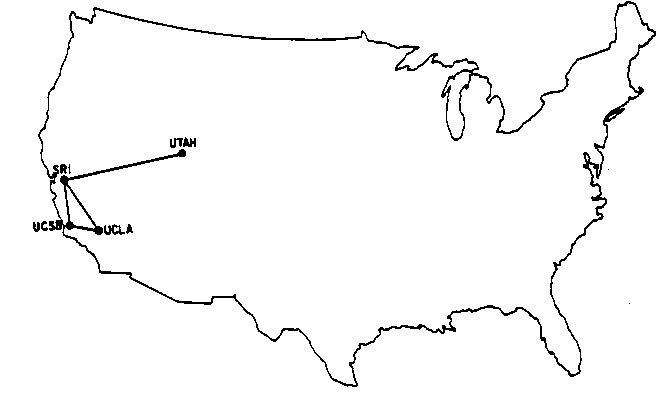
\includegraphics[width=0.4\textwidth]{bib/early_arpanet}}
  \hfill
  \subfloat[More sites connected to the ARPANET, September 1977]{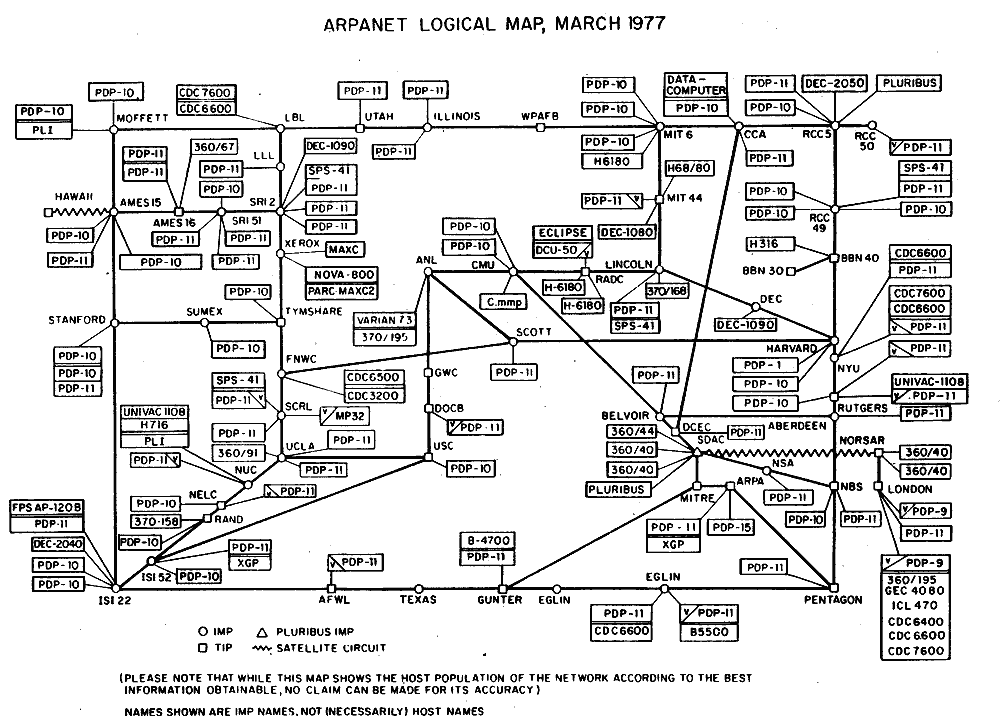
\includegraphics[width=.5\textwidth]{bib/later_arpanet}}
  \caption {ARPANET evolution}
  \label{fig:arpa}
\end{figure}

\par As the advantages of having an interconnected network of computers became clearer, and with the surge of some others, 
such as CYCLADES, the french investigation research network, the need to connect the existing networks was rising, 
and that was one of the first steps of creating a global network, later known as the Internet. Some of the essential mechanisms that can still be found to this day were also developed in the ARPANET, like FTP and e-mail.

\par One of them was introduced in 1981, RFC 793 \cite{postel_transmission_1981}, and with it TCP was "invented".
The main motivation for this development was the introduction of an end-to-end, connection oriented, and reliable protocol that allowed for the standardization of 
several different protocols. Also in this document, the definition of a OSI model, like the one that is prevalent today, or the definitions of reliability, are present, and continue
to be relevant until today.

\begin{figure}[!tbph]
  \centering
  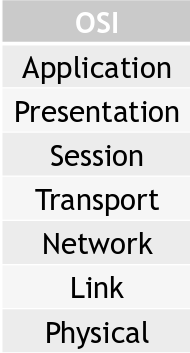
\includegraphics[width=0.2\textwidth]{bib/osi_model}
  \label{fig:osi_model}
  \caption{The current OSI model}
\end{figure}

%%COMECAR A INTRODUZIR WIFI 
One 

\subsection {Market data}
\hspace {5mm} 

%%CISCO REPORT: https://www.cisco.com/c/en/us/solutions/collateral/service-provider/visual-networking-index-vni/vni-hyperconnectivity-wp.html
\par By continuing to evolve and increase in both functionalities and users, the Internet as we know it is a global network, encompassing several protocols, and allows for instant communication of people around the world.
A report indicating this evolution allows for some interesting conclusions about the state of the Internet market until 2021. This forecast was developed based on data originating from projections made from some 
Telecom and Media groups, direct data collection, and some estimates.  \begin {description} \item [Global IP traffic] As the report mentions, the monthly traffic, per capita, in 2016 is around 13 GB, and in 2021 is projected to be at 35 GB
    \item [Mobile devices traffic] While today wired devices still make up for the majority of IP traffic, in 2021, traffic originating from Wi-Fi and mobile devices should account for 63 percent of the total traffic
    \item [Smartphone/ PC traffic] By comparing the predicted evolution of smartphone/ pc traffic, the trends indicate that smartphone traffic should exceed fixed PC traffic.
\end {description}

\par The previous points while obvious estimations, show a clear evolution in the way that Internet is usually accessed, and that is the 

%%Trends in cloud datacenters/ cloud environments

\par 

\section {Software Defined Networking}
\hspace {5mm}
 As described in the previous section, there is a clear evolution of requirements, and this evolution was possible due to the adaptation of the exiting technologies to support better, and more efficient protocols that could carry 
the large amount of data that is transmitted every second. With that in mind, and in order to reduce costs to the service providers, simplify deployment and maintenance operations, developments in Software-Defined Networking (SDN) and Network Function Virtualization have been growing since 2010.

\par This new paradigm introduces programmability in the configuration and management of networks, by consolidating the control of network devices to a single central controller, achieving separation of the control and the 
data plane, and supporting a more dynamic and flexible infrastructure. Another important paradigm, that follows the development of SDN, is the concept of Network Function Virtualization. This concept allows to remove the amount of 
        \textit {middleboxes}\footnote {Computer networking device that does some operations on traffic, excepting packet forwarding. Examples include caches, IDS's, NAT's, ..}, by replacing these with generic software 
applications.

\par The essence of SDN/NFV is described in a short manner if the Open Networking Foundation (ONF) paper: \textit{ In the SDN architecture, the control and data planes are decoupled,  network intelligence and state are 
logically centralized, and the underlying network infrastructure is abstracted from the applications}. The following picture defines both of the approaches to network, the traditional one, where the data and control plane
are just one, and the SDN way, that considers that application and control traffic should be considered in two different ways. 

\begin{figure}[!tbph]
  \centering
  \subfloat[Traditional networking architecture]{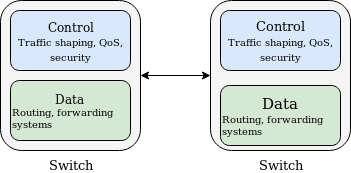
\includegraphics[width=0.4\textwidth]{bib/network_trad}\label{fig:net_trad}}
  \hfill
  \subfloat[SDN architecture]{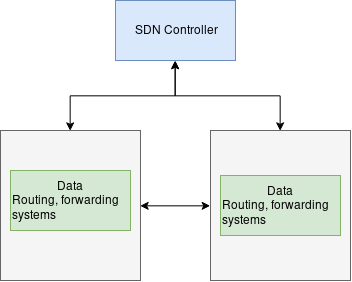
\includegraphics[width=.4\textwidth]{bib/network_sdn}\label{fig:net_sdn}}
  \caption {Traditional vs SDN network architecture}
\end{figure}

\pagebreak

\par One example of the operation of a switch in the SDN model is the following:

\begin {itemize} 
    \item A switch runs an agent, and this agent is connected to a controller;
    \item This controller runs software that can operate the network, managing flow control rules, and collecting information, enabling a full view of the network from a central node
    \item While this controller can be logically centralized, for fault-tolerance and high availability purposes it can be distributed, and by optimizing datamodels and providing caches, one of the earliest ONOS prototypes was
able to achieve a distributed Network OS that could be applied to production networks \cite {berde_onos:_2014}
\end {itemize}

\par More details on the technology that runs this model can be found in the next chapter. 
\par After analysing some examples of deployment of the SDN model, the analysed literature provides some insights on the requirements that platforms using this paradigm need to obey \cite {masutani_requirements_2014}.
 
\begin {itemize} 
    \item \textbf{High Performance}   
    \item \textbf{High Availability} 
    \item \textbf{Fault Tolerance}   
    \item \textbf{Monitoring}   
    \item \textbf{Programmability}   
    \item \textbf{Security}   
\end {itemize}



\subsection {Why?}
\subsection {Challenges}
\subsection {Observed implementations in the industry}

\section {Cloud Computing}
\section {Databases} 

